\documentclass[hidelinks,12pt]{article}
\usepackage[left=0.25cm,top=1cm,right=0.25cm,bottom=1cm]{geometry}
%\usepackage[landscape]{geometry}
\textwidth = 20cm
\hoffset = -1cm
\usepackage[utf8]{inputenc}
\usepackage[spanish,es-tabla]{babel}
\usepackage[autostyle,spanish=mexican]{csquotes}
\usepackage[tbtags]{amsmath}
\usepackage{nccmath}
\usepackage{amsthm}
\usepackage{amssymb}
\usepackage{mathrsfs}
\usepackage{graphicx}
\usepackage{subfig}
\usepackage{standalone}
\usepackage[outdir=./Imagenes/]{epstopdf}
\usepackage{siunitx}
\usepackage{physics}
\usepackage{color}
\usepackage{float}
\usepackage{hyperref}
\usepackage{multicol}
%\usepackage{milista}
\usepackage{anyfontsize}
\usepackage{anysize}
%\usepackage{enumerate}
\usepackage[shortlabels]{enumitem}
\usepackage{capt-of}
\usepackage{bm}
\usepackage{relsize}
\usepackage{placeins}
\usepackage{empheq}
\usepackage{cancel}
\usepackage{wrapfig}
\usepackage[flushleft]{threeparttable}
\usepackage{makecell}
\usepackage{fancyhdr}
\usepackage{tikz}
\usepackage{bigints}
\usepackage{scalerel}
\usepackage{pgfplots}
\usepackage{pdflscape}
\pgfplotsset{compat=1.16}
\spanishdecimal{.}
\renewcommand{\baselinestretch}{1.5} 
\renewcommand\labelenumii{\theenumi.{\arabic{enumii}})}
\newcommand{\ptilde}[1]{\ensuremath{{#1}^{\prime}}}
\newcommand{\stilde}[1]{\ensuremath{{#1}^{\prime \prime}}}
\newcommand{\ttilde}[1]{\ensuremath{{#1}^{\prime \prime \prime}}}
\newcommand{\ntilde}[2]{\ensuremath{{#1}^{(#2)}}}

\newtheorem{defi}{{\it Definición}}[section]
\newtheorem{teo}{{\it Teorema}}[section]
\newtheorem{ejemplo}{{\it Ejemplo}}[section]
\newtheorem{propiedad}{{\it Propiedad}}[section]
\newtheorem{lema}{{\it Lema}}[section]
\newtheorem{cor}{Corolario}
\newtheorem{ejer}{Ejercicio}[section]

\newlist{milista}{enumerate}{2}
\setlist[milista,1]{label=\arabic*)}
\setlist[milista,2]{label=\arabic{milistai}.\arabic*)}
\newlength{\depthofsumsign}
\setlength{\depthofsumsign}{\depthof{$\sum$}}
\newcommand{\nsum}[1][1.4]{% only for \displaystyle
    \mathop{%
        \raisebox
            {-#1\depthofsumsign+1\depthofsumsign}
            {\scalebox
                {#1}
                {$\displaystyle\sum$}%
            }
    }
}
\def\scaleint#1{\vcenter{\hbox{\scaleto[3ex]{\displaystyle\int}{#1}}}}
\def\bs{\mkern-12mu}



\title{Funciones ordinarias de Laguerre \\ \large {Tema 5 - Funciones especiales} \vspace{-3ex}}
\author{M. en C. Gustavo Contreras Mayén}
\date{ }

\pagestyle{fancy}
\fancyhf{}
\rhead{Curso MAF}
\lhead{\leftmark}
\rfoot{\thepage}
\setlength{\headheight}{16pt}%

\def\changemargin#1#2{\list{}{\rightmargin#2\leftmargin#1}\item[]}
\let\endchangemargin=\endlist 


\begin{document}
\maketitle
\fontsize{14}{14}\selectfont
\tableofcontents
\newpage

%Referencia: Griffits - 4.2 The hydrogen atom

\section{El átomo de hidrógeno.}

El átomo de hidrógeno consta de un protón pesado, esencialmente inmóvil (de tal manera que podemos ponerlo en el origen) de carga $e$, junto con un electrón mucho más ligero (de carga $-e$) que se desplaza en círculo alrededor del protón, y se mantiene en órbita por la atracción mutua de cargas opuestas (ver Figura \ref{fig:figura_01}).
\begin{figure}[H]
    \centering
    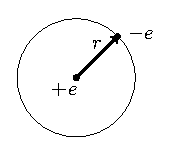
\includegraphics[scale=1.5]{Imagenes/atomohidrogeno.eps}
    \caption{El átomo de hidrógeno.}
    \label{fig:figura_01}
\end{figure}
A partir de la ley de Coulomb, la energía potencial (en unidades SI) es:
\begin{align}
V(r) = - \dfrac{e^{2}}{4 \, \pi \, \epsilon_{0}} \; \dfrac{1}{r}
\label{eq:ecuacion_04_52}
\end{align}
y la ecuación radial es:
\begin{align}
- \dfrac{\hbar^{2}}{2 \, m} \; \dv[2]{u}{r} + \left[ - \dfrac{e^{2}}{4 \, \pi \, \epsilon_{0}} \; \dfrac{1}{r} + \dfrac{\hbar^{2}}{2 \, m} \; \dfrac{\ell(\ell +1)}{r^{2}} \right] \, u =  E \, u
\label{eq:ecuacion_04_53}
\end{align}

Nuestro problema es resolver esta ecuación para $u(r)$ y determinar las energías permitidas $E$ de los electrones. 
\par
El potencial de Coulomb (ec. \ref{eq:ecuacion_04_52}) admite estados de medios continuos (con $E > 0$), la descripción de electrones la dispersión de protones, así como estados ligados discretos, lo que representa el átomo de hidrógeno, pero nos limitaremos nuestra atención a este último.

\subsection{La función radial de onda.}

Nuestra primera tarea es poner en orden la notación. Dejando:
\begin{align}
\kappa \equiv \dfrac{\sqrt{-2 \, m \, E}}{\hbar}
\label{eq:ecuacion_04_54}
\end{align}
(Para estados base, $E < 0$, por lo que $\kappa$ es real). Al dividir la ec. (\ref{eq:ecuacion_04_53}) por $E$, tenemos:
\begin{align*}
\dfrac{1}{\kappa^{2}} \, \dv{2}{u}{r} = \left[1 - \dfrac{m \, e^{2}}{2 \, \pi \, \epsilon_{0} \,\hbar^{2} \kappa} \, \dfrac{1}{(\kappa \, r)} + \dfrac{\ell (\ell + 1)}{(\kappa \, r)^{2}} \right] \, u
\end{align*}
donde podemos hacer:
\begin{align}
\rho \equiv \kappa \, r \hspace{1cm} \rho_{0} \equiv \dfrac{m \, e^{2}}{2 \, \pi \, \epsilon_{0} \, \hbar^{2} \, \kappa}
\label{eq:ecuacion_04_55}
\end{align}
por lo que:
\begin{align}
\dv[2]{u}{\rho} = \left[ 1 - \dfrac{\rho_{0}}{\rho} + \dfrac{\ell (\ell + 1)}{\rho^{2}} \right] \, u
\label{eq:ecuacion_04_56}
\end{align}
Revisemos la forma asintótica de las soluciones: mientras $\rho \to \infty$, el término constante en los paréntesis es el que domina, por lo que aproximadamente:
\begin{align*}
\dv[2]{u}{\rho} = u
\end{align*}
La solución general es del tipo:
\begin{align}
u(\rho) = A \, e^{-\rho} + B \, e^{\rho}
\label{eq:ecuacion_04_57}
\end{align}
pero $exp(\rho)$ se anula cuando $\rho \to \infty$, así $B = 0$, evidentemente:
\begin{align}
u(\rho) \sim A \, e^{-\rho}
\label{eq:ecuacion_04_58}
\end{align}
para valores grandes de $\rho$. Mientras que por otro lado, mientras que $\rho \to 0$ el término centrífugo domina, por lo que la aproximación es:
\begin{align*}
\dv[2]{u}{\rho} = \dfrac{\ell (\ell + 1)}{\rho^{2}} \, u
\end{align*}
que tiene por solución general:
\begin{align*}
u(\rho) = C \, \rho^{\ell +1} + D \, \rho^{-\ell}
\end{align*}
pero el término $\rho^{-\ell}$ se anula cuando $\rho \to 0$, así $D = 0$, por lo que:
\begin{align}
u(\rho) \sim C \, \rho^{\ell + 1}
\label{eq:ecuacion_04_59}
\end{align}
para valores pequeños de $\rho$.
\par
El siguiente paso es revisar el comportamiento asintótico, al introducir una nueva función $v(\rho)$:
\begin{align}
u(\rho) = \rho^{\ell + 1} \, e^{-\rho} \, v(\rho)
\label{eq:ecuacion_04_60} 
\end{align}
en espera que $v(\rho)$ sea tan sencilla como $u(\rho)$, pero la primera vista nos dice que en apariencia, no es así:
\begin{align*}
\dv{u}{\rho} = \rho^{\ell} \, e^{-\rho} \left[ (\ell + 1 - \rho) \, v + \rho \, \dv{v}{\rho} \right]
\end{align*}
y
\begin{align*}
\dv[2]{u}{\rho} = \rho^{\ell} \, e^{-\rho} \left( \left[ -2 \, \ell - 2 + \rho + \dfrac{ \ell (\ell + 1)}{\rho} \right] \, v + 2 (\ell + 1 - \rho) \, \dv{v}{\rho} + \rho \dv[2]{v}{\rho} \right)
\end{align*}
en términos de $v(\rho)$, la ecuación radial (ec. \ref{eq:ecuacion_04_56}) se escribe:
\begin{align}
\rho \, \dv[2]{v}{\rho} + 2 (\ell + 1 - \rho) \dv{v}{\rho} + [\rho_{0} - 2 (\ell + 1)] \, v = 0
\label{eq:ecuacion_04_61}
\end{align}
Finalmente, suponemos que la solución $v(\rho)$ puede expresarse como una serie de potencias en $\rho$:
\begin{align}
v(\rho) = \sum_{j=0}^{\infty} a_{j} \, \rho^{j} 
\label{eq:ecuacion_04_62}
\end{align}
Nuestro problema ahora es determinar los coeficientes $(a_{0}, a_{1}, a_{2}, \ldots)$. Diferenciando término a término:
\begin{align*}
\dv{v}{\rho} = \sum_{j=0}^{\infty} j \, a_{j} \, \rho^{j - 1} = \sum_{j=0}^{\infty} (j + 1) \, a_{j+1} \, \rho^{j}
\end{align*}
En la segunda suma, se ha renombrado el índice mudo $j \to j + 1$. Diferenciando nuevamente:
\begin{align*}
\dv[2]{v}{\rho} = \sum_{j=0}^{\infty} j \, (j+1) \, a_{j+1} \, \rho^{j-1}
\end{align*}
sustituyendo en la ecuación (\ref{eq:ecuacion_04_61}), tenemos:
\begin{align*}
\sum_{j=0}^{\infty} j \, (j &+ 1) \, a_{j+1} \, \rho^{j} + 2 (\ell + 1) \, \sum_{j=0}^{\infty} (j + 1) \, a_{j+1} \rho^{j} + \\[0.5em]
&- 2 \sum_{j=0}^{\infty} j \, a_{j} \, \rho^{j} + [ \rho_{0} - 2 \, (\ell + 1)] \sum_{j=0}^{\infty} a_{j} \, \rho^{j} = 0
\end{align*}
igualando los coeficientes de las potencias similares, nos lleva a:
\begin{align*}
j \, (j + 1) \, a_{j+1} + 2(\ell + 1)(j + 1) \, a_{j+1} - 2 \, j \, a_{j} + [\rho_{0} - 2(\ell + 1)] \, a_{j} = 0
\end{align*}
o equivalentemente:
\begin{align}
a_{j+1} = \left[ \dfrac{2 \, (j + \ell + 1) - \rho_{0}}{(j + 1)(j + 2 \, \ell + 2)} \right] \, a_{j}
\label{eq:ecuacion_04_63}
\end{align}
Esta fórmula de recurrencia determina los coeficientes, y por lo tanto la función $v(\rho)$: Comenzamos con $a_{0}$ (esto se convierte en una constante en general, que se fija por la normalización), y la ecuación (\ref{eq:ecuacion_04_63}) nos devuelve $a_{1}$, usando este valor, se obtiene un $a_{2}$, y así.
\par
Ahora vamos a ver a qué se parecen los coeficientes grandes $j$ (esto corresponde a un valor grande de $\rho$, donde dominan las potencias superiores). En este régimen la fórmula de recurrencia nos dice que:
\begin{align*}
a_{j+1} \cong \dfrac{2 \, j}{j (j + 1)} \, a_{j} =  \dfrac{2}{j + 1} \, a_{j}
\end{align*}
así:
\begin{align}
a_{j} \cong \dfrac{2^{j}}{j!} \, A
\label{eq:ecuacion_04_64}
\end{align}
Suponemos que éste es el valor exacto, así:
\begin{align*}
v(\rho) = A \, \sum_{j=0}^{\infty} \dfrac{2^{j}}{j!} =  A \, e^{2 \rho}
\end{align*}
por tanto:
\begin{align}
u(\rho) = A \, \rho^{\ell + 1} \, e^{\rho}
\label{eq:ecuacion_04_65}
\end{align}
que \enquote{vuela} para valores grandes de $\rho$. El exponencial positivo es precisamente el comportamiento asintótico que no queríamos en la ecuación (\ref{eq:ecuacion_04_57}). (No es ningún accidente que ha vuelto a aparecer, después de todo sí representa la forma asintótica de algunas soluciones a la ecuación radial que simplemente no resultan ser los que estamos interesados, porque no son normalizables.
\par
Sólo hay una manera de salir de este dilema: \emph{La serie debe terminar}. Tiene que haber algún entero máximo, $j_{\text{max}}$, de tal manera que
\begin{align}
a_{j_{\text{max} + 1}} = 0
\label{eq:ecuacion_04_66}
\end{align}
(Y más allá del cual todos los coeficientes desaparecen automáticamente). Evidentemente (ec. \ref{eq:ecuacion_04_63}):
\begin{align*}
2 \, (j_{\text{max}} + \ell + 1) - \rho_{0} = 0
\end{align*}
Definimos:
\begin{align}
n \equiv j_{\text{max}} + \ell + 1
\label{eq:ecuacion_04_67}
\end{align}
(que llamaremos \textbf{número cuántico principal}), tenemos que:
\begin{align}
\rho_{0} = 2 \, n
\label{eq:ecuacion_04_68}
\end{align}
Pero $\rho_{0}$ determina la $E$ (ecs. \ref{eq:ecuacion_04_54} y \ref{eq:ecuacion_04_55}):
\begin{align}
E = - \dfrac{\hbar^{2} \, \kappa^{2}}{2 \, m} = - \dfrac{m \, e^{2}}{8 \, \pi^{2} \, \epsilon_{0}^{2} \, \hbar^{2} \, \rho_{0}^{2}}
\label{eq:ecuacion_04_69}
\end{align}
y las energías permitidas son:
\begin{align}
\setlength{\fboxsep}{3\fboxsep}\boxed{
E_{n} = - \left[ \dfrac{m}{2 \, \hbar^{2}} \left( \dfrac{e^{2}}{4 \, \pi \, \epsilon_{0}} \right)^{2} \right] \dfrac{1}{n^{2}} = \dfrac{E_{1}}{n^{2}}, \hspace{1cm} n = 1, 2, 3, \ldots}
\label{eq:ecuacion_04_70}
\end{align}
Esta es la famosa fórmula de Bohr, para cualquier medida, es el resultado más importante de toda la mecánica cuántica. Bohr lo obtuvo en 1913 por una mezcla casual de una inaplicable física clásica y una teoría cuántica prematura (la ecuación de Schrödinger no llegó hasta 1924).
\par
Combinando las ecuaciones (\ref{eq:ecuacion_04_55}) y (\ref{eq:ecuacion_04_68}), encontramos que:
\begin{align}
\kappa = \left( \dfrac{m \, e^{2}}{4 \, \pi \, e_{0} \, \hbar^{2}} \right) \dfrac{1}{n} = \dfrac{1}{a \, n}
\label{eq:ecuacion_04_71}
\end{align}
donde:
\begin{align}
\setlength{\fboxsep}{3\fboxsep}\boxed{
a \equiv \dfrac{4 \, \pi \, \epsilon_{0} \, \hbar^{2}}{m \, e^{2}} = \SI{0.529e-10}{\metre}}
\label{eq:ecuacion_04_72}
\end{align}
al que se le denomina \emph{radio de Bohr}. Se sigue (de la ec. \ref{eq:ecuacion_04_55}) que:
\begin{align}
\rho = \dfrac{r}{a \, n}
\label{eq:ecuacion_04_73}
\end{align}
Evidentemente las funciones de onda espaciales para el hidrógeno se etiquetan con tres números cuánticos ($n$, $\ell$ y $m$):
\begin{align}
\psi_{n \ell m} (r, \theta, \phi) =  R_{n \ell} (r) Y_{\ell}^{m} (\theta, \phi)
\label{eq:ecuacion_04_74}
\end{align}
retomando la ecuación (\ref{eq:ecuacion_04_60}):
\begin{align}
R_{n \ell}(r) = \dfrac{1}{r} \, \rho^{\ell + 1} \, e^{-\rho} \, v(\rho)
\label{eq:ecuacion_04_75}
\end{align}
y $v(r\rho)$ es un polinomio de grado $j_{\text{max}} = n - \ell - 1)$ en $\rho$, donde los coeficientes están determinados (hasta un factor de normalización global) por la fórmula de recursión:
\begin{align}
a_{j+1} = \dfrac{2 (j + \ell + 1 - n}{(j + 1)(j + 2 \ell + 2)} a_{j}
\label{eq:ecuacion_04_76}
\end{align}
El \textbf{estado base} (es decir, el estado de menor energía) es el caso cuando $n = 1$, usando los valores de las constantes físicas, se obtiene:
\begin{align}
E_{1} = - \left[ \dfrac{m}{2 \, \hbar^{2}} \left( \dfrac{e^{2}}{4 \, \pi \, \epsilon_{0}} \right)^{2} \right] =  \SI{-13.6}{\electronvolt}
\label{eq:ecuacion_04_77}
\end{align}
Evidentemente, la \textbf{energía de enlace} del hidrógeno (la cantidad de energía que tendría que impartir el electrón con el fin de ionizar el átomo) es de $\SI{13.6}{\electronvolt}$. La ec. (\ref{eq:ecuacion_04_67}) obliga que $\ell = 0$, de donde también $m = 0$, por lo que:
\begin{align}
\psi_{100} (r, \theta, \phi) = R_{10}(r) \, Y_{0}^{0} (\theta, \psi)
\label{eq:ecuacion_04_78}
\end{align}
La fórmula de recursión se trunca después del primer término (ec. \ref{eq:ecuacion_04_76} con $j=0$ devuelve $a_{1} = 0$), así $v(\rho)$ es una constante ($a_{0}$) y:
\begin{align}
R_{10} = \dfrac{a_{0}}{a} \, e^{-r/a}
\label{eq:ecuacion_04_79}
\end{align}
Normalizando:
\begin{align*}
\int_{0}^{\infty} \abs{R_{10}}^{2} \, r^{2} \dd{r} = \dfrac{\abs{a_{0}}^{2}}{a^{2}} \, \int_{0}^{\infty} e^{-2r/a} \, r^{2} \dd{r} =  \abs{a_{0}}^{2} \, \dfrac{a}{4} =  1
\end{align*}
por lo que $a_{0} = 2 / \sqrt{a}$. Mientras que $Y_{0}^{0} = 1 / \sqrt{4 \, \pi}$, así:
\begin{align}
\setlength{\fboxsep}{3\fboxsep}\boxed{
\psi_{100} (r, \theta, \phi) = \dfrac{1}{\sqrt{\pi \, a^{3}}} e^{-r/a}}
\label{eq:ecuacion_04_80}
\end{align}
Si $n = 2$ la energía es:
\begin{align}
E_{2} = \dfrac{\SI{-13.6}{\electronvolt}}{4} =  \SI{- 3.4}{\electronvolt}
\label{eq:ecuacion_04_81}
\end{align}
este es el primer estado excitado, o más bien, \textit{estados}, ya que podemos tener ya sea $\ell = 0$ (en cuyo caso $m = 0$) o $\ell = 1$ (con $m = -1$, $0$, $+ 1$), por lo que son en realidad cuatro estados diferentes que comparten esta energía. Si $\ell = 0$, la relación de recurrencia (ec. \ref{eq:ecuacion_04_76}) da:
\begin{align*}
a_{1} = - a_{0} \hspace{0.5cm} \text{(usando } j = 0 \text{)}, \hspace{1.5cm} \text{y } a_{2} = 0 \hspace{0.5cm} \text{(usando } j = 1 \text{)}
\end{align*}
así $v(\rho) = a_{0} \, (1 - \rho)$, y por tanto:
\begin{equation}
R_{20}(r) = \dfrac{a_{0}}{2 \, a} \left(1 - \dfrac{r}{2 \, a} \right) e^{-r/2a}
\label{eq:ecuacion_04_82}
\end{equation}
Si $\ell = 1$ la fórmula de recurrencia termina la serie luego de un solo término, así $v(\rho)$ es una constante, por lo que se encuentra que:
\begin{align}
R_{21}(r) = \dfrac{a_{0}}{4 \, a^{2}} \; r e^{-r/2a}
\label{eq:ecuacion_04_83}
\end{align}
En cada caso la constante $a_{0}$, está determinado por la normalización.
\par
Para un valor arbitrario de $n$, los posibles valores de $\ell$, son:
\begin{align}
\ell = 0, 1, 2, \ldots, n - 1
\label{eq:ecuacion_04_84}
\end{align}
Para cada $\ell$, existen $2 \, \ell + 1$ valores posibles de $m$, por lo que el nivel total de energía degenerada $E_{n}$ es:
\begin{align}
d(n) = \sum_{\ell = 0}^{n - 1} (2 \, \ell + 1) = n^{2}
\label{eq:ecuacion_04_85}
\end{align}
la función polinomial $v(\rho)$ es una función conocida de la matemática, se puede escribir como:
\begin{align}
v(\rho) = L_{n-\ell-1}^{2\ell+1}(2 \, \rho)
\label{eq:ecuacion_04_86}
\end{align}
donde:
\begin{align}
L_{q-p}^{p} (x) = (-1)^{p} \left( \dv{x} \right)^{p} L_{q}(x)
\label{eq:ecuacion_04_87}
\end{align}
son los \textbf{polinomios asociados de Laguerre} y:
\begin{align}
L_{q}(x) = e^{x} \left( \dv{x} \right)^{q} \; (e^{-x} \; x^{q})
\label{eq:ecuacion_04_88}
\end{align}
es el \textbf{polinomio ordinario de Laguerre de orden $n$}.
En la tabla (\ref{table:tabla_01}) se muestran los primeros polinomios de Laguerre $L_{q}(x)$, mientras que en la tabla (\ref{table:tabla_02}) se muestran algunos polinomios asociados de Laguerre $L_{q-p}^{p}(x)$.
\begin{table}[H]
\centering
\large
\begin{tabular}{l}
$L_{0} (x) = 1$ \\
$L_{1} (x) = - x + 1$ \\
$L_{2} (x) = x^{2} - 4 \, x + 2$ \\
$L_{3} (x) = - x^{3} + 9 \, x^{2} - 18 \, x + 6$ \\
\vdots 
\end{tabular}
\caption{Primeros polinomios ordinarios de Laguerre.}
\label{table:tabla_01}
\end{table}
\begin{figure}[H]
    \centering
    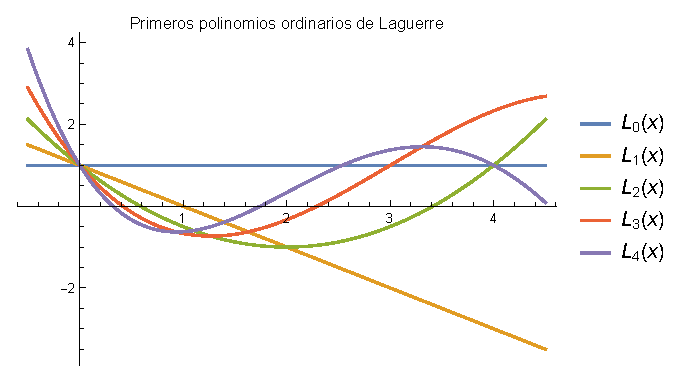
\includegraphics[scale=1.2]{Imagenes/Polinomios_Laguerre_01.eps}
    \caption{Gráfica con los primeros polinomios ordinarios de Laguerre.}
    \label{fig:grafica_Laguerre_01}
\end{figure}
A continuación se presenta una lista con los primeros polinomios asociados de Laguerre y una gráfica:
\begin{table}[H]
\centering
\large
\begin{tabular}{l l}
$L_{0}^{0} (x) = 1$ & $L_{0}^{2} = 2$  \\
$L_{1}^{0} (x) = - x + 1$ & $L_{1}^{2} = -6 \, x + 18$ \\
$L_{2}^{0} (x) = x^{2} - 4 x + 2$ & $L_{2}^{2} = 12 \, x^{2} - 96 \, x + 144$ \\
$L_{0}^{1} (x) = 1$ & $L_{0}^{3} = 6$ \\
$L_{1}^{1} (x) = -2x + 4$ & $L_{1}^{3} = -24 \, x + 96$ \\
\vdots 
\end{tabular}
\caption{Primeros polinomios asociados de Laguerre.}
\label{table:tabla_02}
\end{table}
\begin{figure}[H]
    \centering
    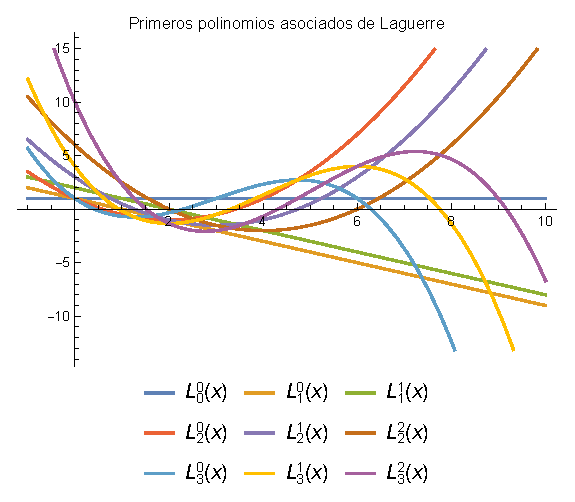
\includegraphics[scale=1.2]{Imagenes/Polinomios_Laguerre_02.eps}
    \caption{Gráfica con los primeros polinomios asociados de Laguerre.}
    \label{fig:grafica_Laguerre_02}
\end{figure}
Las funciones de onda normalizadas para el hidrógeno son:
\begin{align}
\setlength{\fboxsep}{3\fboxsep}\boxed{
\psi_{n \ell m} = \sqrt{\left(\dfrac{2}{n \, a} \right)^{3} \dfrac{(n - \ell - 1)}{2 \, n[(n + \ell)!]^{3}}} e^{-r/na} \; \left( \dfrac{2 \, r}{n \, a} \right)^{\ell} \; L_{n - \ell -1}^{2 \ell + 1} \left( \dfrac{2 \, r}{n \, a} \right) Y_{\ell}^{m} \, (\theta, \phi)}
\label{eq:ecuacion_04_89}
\end{align}
No se miran muy agradables, pero no se quejan, este es uno de los muy pocos sistemas realistas que se puede resolver del todo, de forma exacta. Como verá más adelante, son mutuamente ortogonales:
\begin{align}
\int \psi_{n \ell m}^{*} \psi_{\ptilde{n} \ptilde{\ell} \ptilde{m}} \, r^{2} \, \sin \theta \dd{r} \dd{\theta} \dd{\phi} =  \delta_{n \prime{n}} \delta_{\ell \delta{\ell}} \delta_{m \delta{m}}
\label{eq:ecuacion_04_90}
\end{align}
Esto se debe a la ortogonalidad de los armónicos esféricos y (para $n \neq n$) de que son las funciones propias de $H$ con distinto valor propio.
\par
Visualizar como tal las funciones de onda del hidrógeno no es fácil, a los químicos les agrada usar \enquote{gráficas de densidad}, en las cuales el nivel de brillo de la nube es proporcional a $\abs{\Psi}^{2}$, como se puede ver en la figura\footnote{Tomada con licencia de:  (\ref{fig:figura_espectro_H}) \href{https://commons.wikimedia.org/wiki/File:Hydrogen_Density_Plots.png}{Visita el sitio.}} :
\begin{figure}[H]
    \centering
    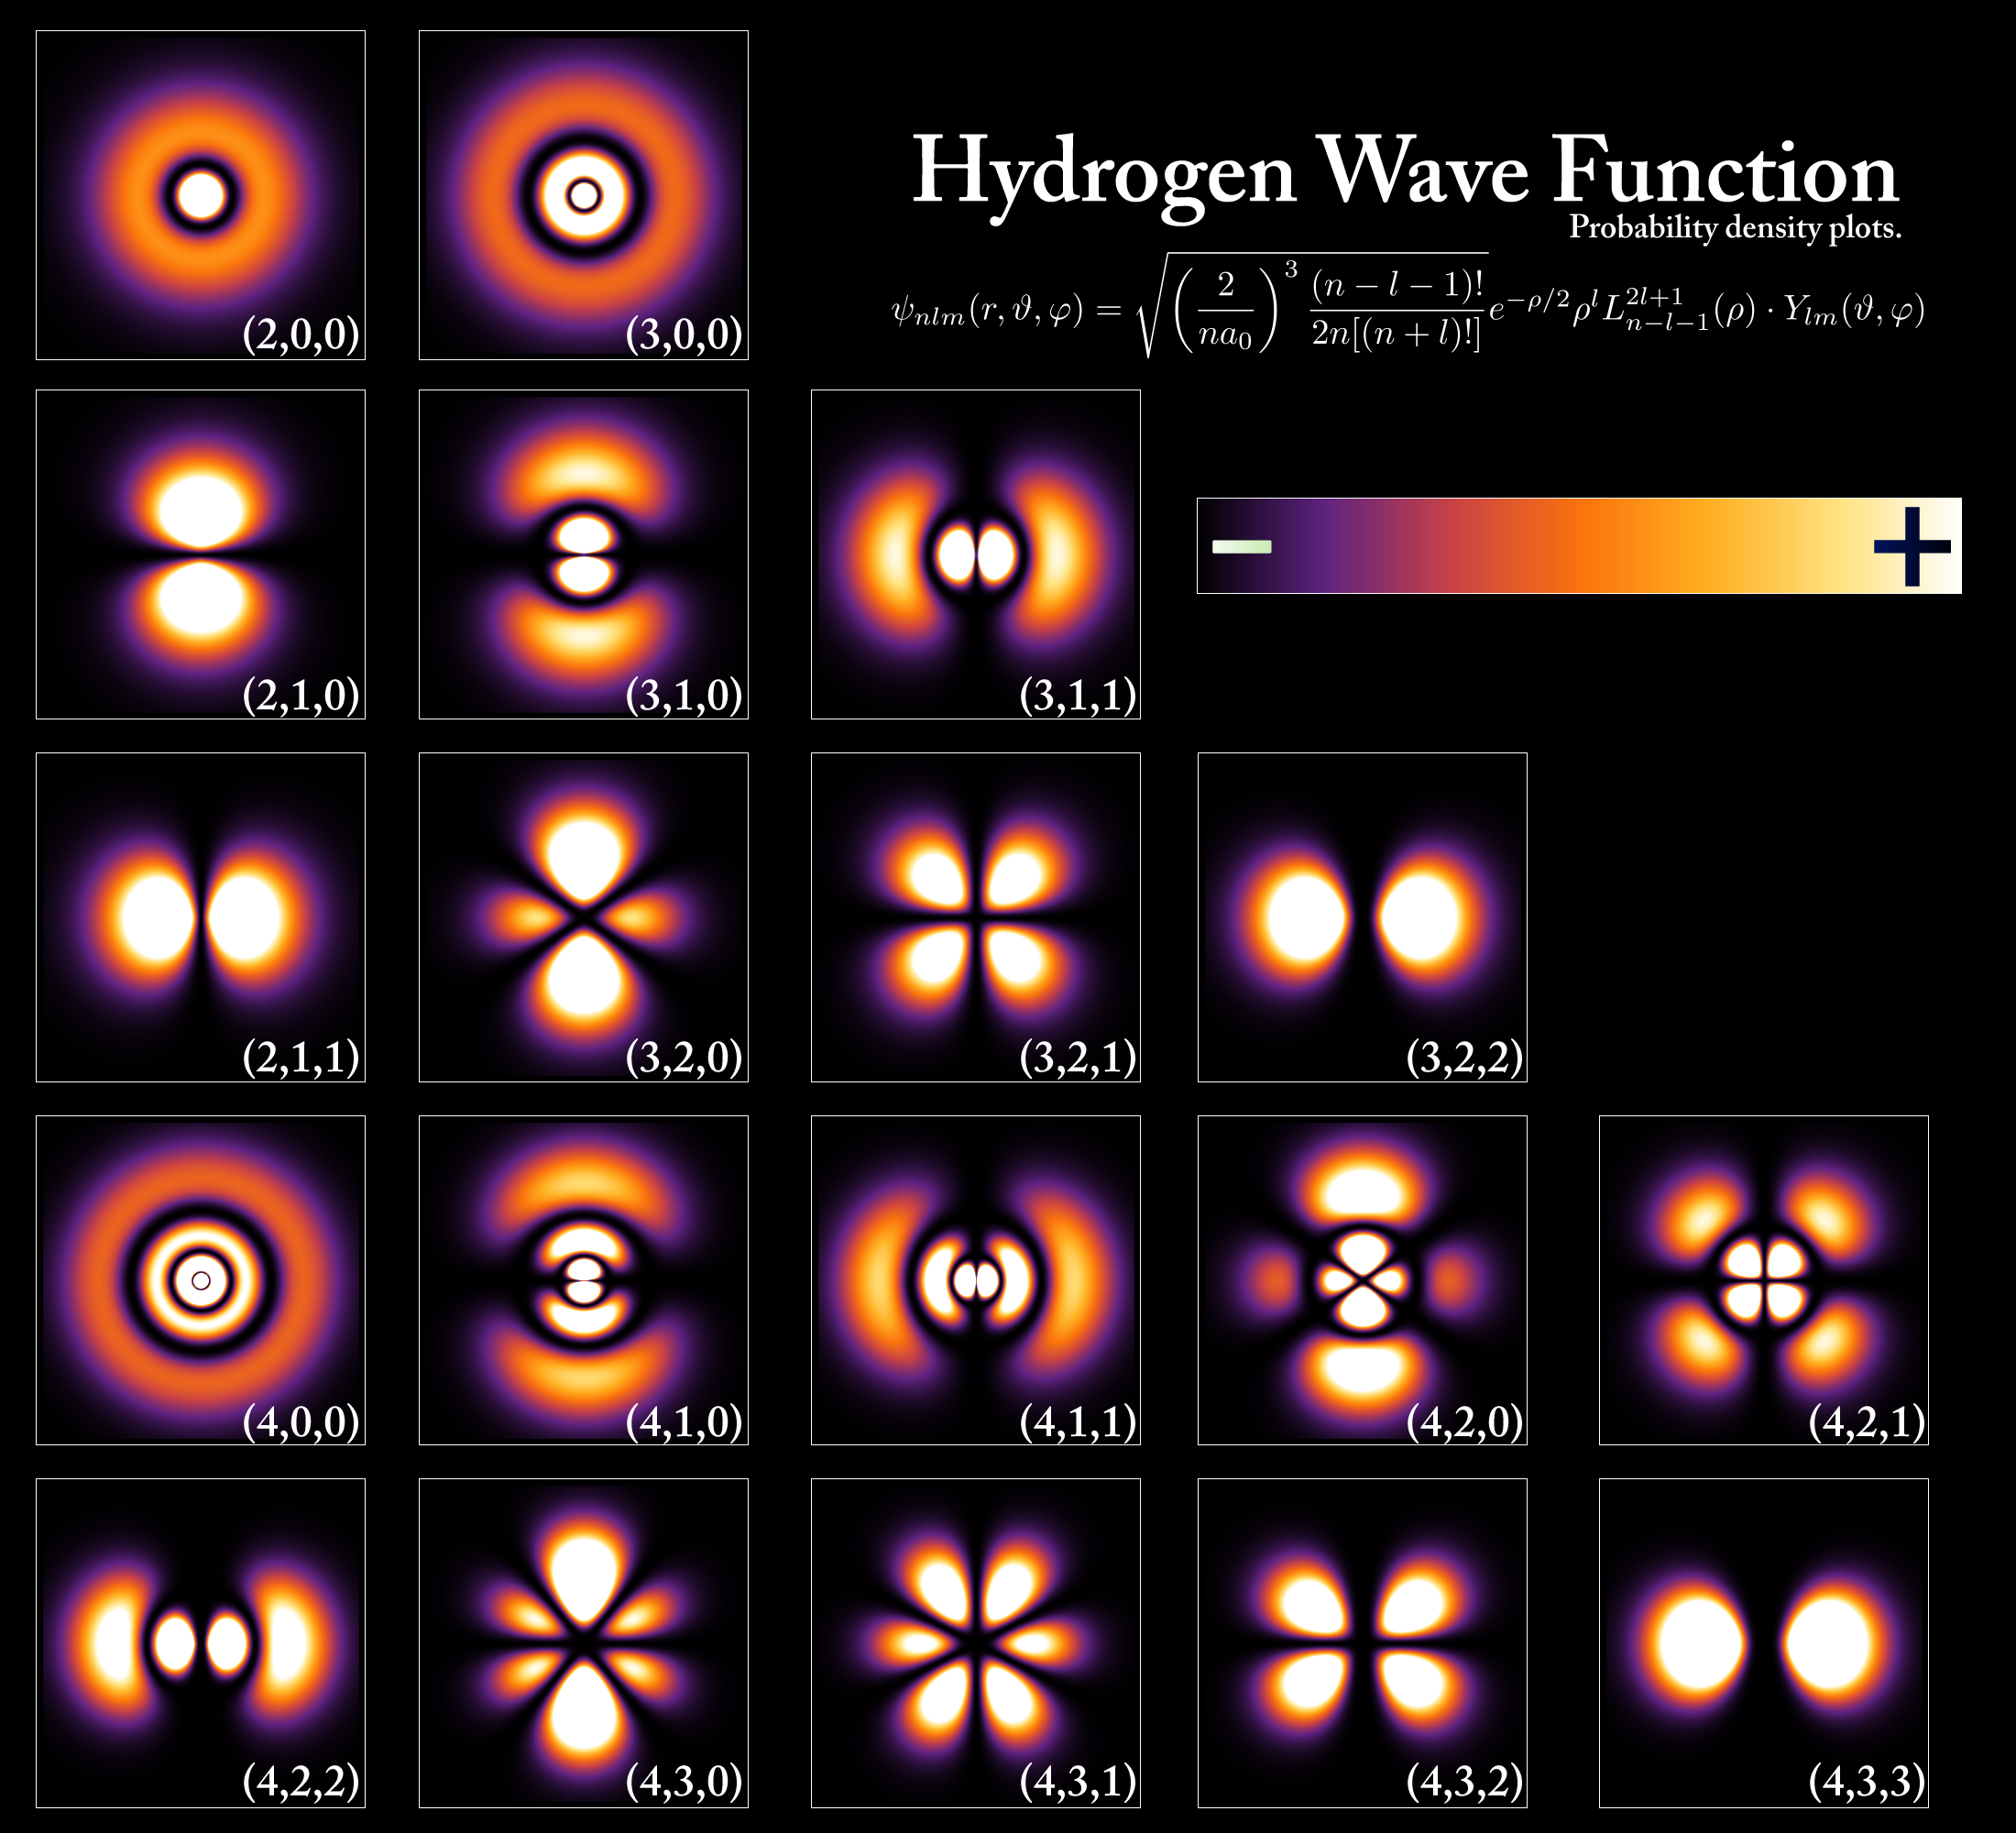
\includegraphics[scale=0.15]{Imagenes/Hydrogen_Density_Plots.png}
    \caption{Gráficas de densidad de estado para el hidrógeno}
\end{figure}


\subsection{Espectro del hidrógeno.}

En principio, si ponemos un átomo de hidrógeno en un estado estacionario $\Psi_{n \ell m}$, debe quedarse allí para siempre. Sin embargo, si \emph{perturbamos} ligeramente (por colisión con otro átomo, por ejemplo, o haciéndole incidir  luz en él), entonces el átomo puede experimentar una transición a otro estado estacionario mediante la absorción de la energía y pasarse a un estado de mayor energía o cediendo energía (normalmente en forma de radiación electromagnética) y moverse  hacia abajo.
\par
En la práctica este tipo de perturbaciones están siempre presentes; transiciones (o, como a veces se denominan \enquote{saltos cuánticos}) se producen constantemente, y el resultado es que un contenedor de hidrógeno emite luz (fotones), cuya energía corresponde a la diferencia de energía entre los estados inicial y final:
\begin{align}
E_{\gamma} = E_{i} - E_{f} = \SI{-13.6}{\electronvolt} \left( \dfrac{1}{n_{i}^{2}} - \dfrac{1}{n_{f}^{2}} \right)
\label{eq:ecuacion_04_91}
\end{align}
de acuerdo con la fórmula de Planck, la energía de un fotón es proporcional a su frecuencia:
\begin{align}
E_{\gamma} = h \, \nu
\label{eq:ecuacion_04_92}
\end{align}
Mientras que la longitud de onda está dada por $\lambda = c / \nu)$, por tanto:
\begin{align}
\dfrac{1}{\lambda} = R \left( \dfrac{1}{n_{f}^{2}} - \dfrac{1}{n_{i}^{2}} \right)
\label{eq:ecuacion_04_93}
\end{align}
donde:
\begin{align}
R = \dfrac{m}{4 \, \pi \, c \, \hbar} \left( \dfrac{e^{2}}{4 \, \pi \, \epsilon_{0}} \right)^{2} = \SI{1.097e7}{\per\metre}
\label{eq:ecuacion_04_94}
\end{align}
a $R$ se le conoce como la \textbf{constante de Rydberg}, y la ec. (\ref{eq:ecuacion_04_93}) es la \textbf{fórmula Rydberg} para el espectro de hidrógeno. Fue descubierto empíricamente en el siglo XIX, y el mayor triunfo de la teoría de Bohr fue su capacidad para dar cuenta de este resultado y calcular $R$ en función de las constantes fundamentales de la naturaleza.
\par
Las transiciones al estado base ($n_{f}= 1$) se encuentran en el ultravioleta; son conocidas por los espectroscopistas como la \textbf{serie de Lyman}. Las transiciones al primer estado excitado ($n_{f}= 2$) se encuentran en la zona de región visible; conforman la \textbf{serie de Balmer}. Las transiciones a $n_{f} = 3$ (la \textbf{serie de Paschen}) están en el infrarrojo, y así sucesivamente (véase la figura \ref{fig:figura_espectro_H}). (A temperatura ambiente, la mayoría de los átomos de hidrógeno están en el estado base, para obtener el espectro de emisión, se deben elevar primero los diferentes estados excitados, por lo general esto se realiza haciendo pasar una chispa eléctrica a través del gas.)
\begin{figure}[H]
    \centering
    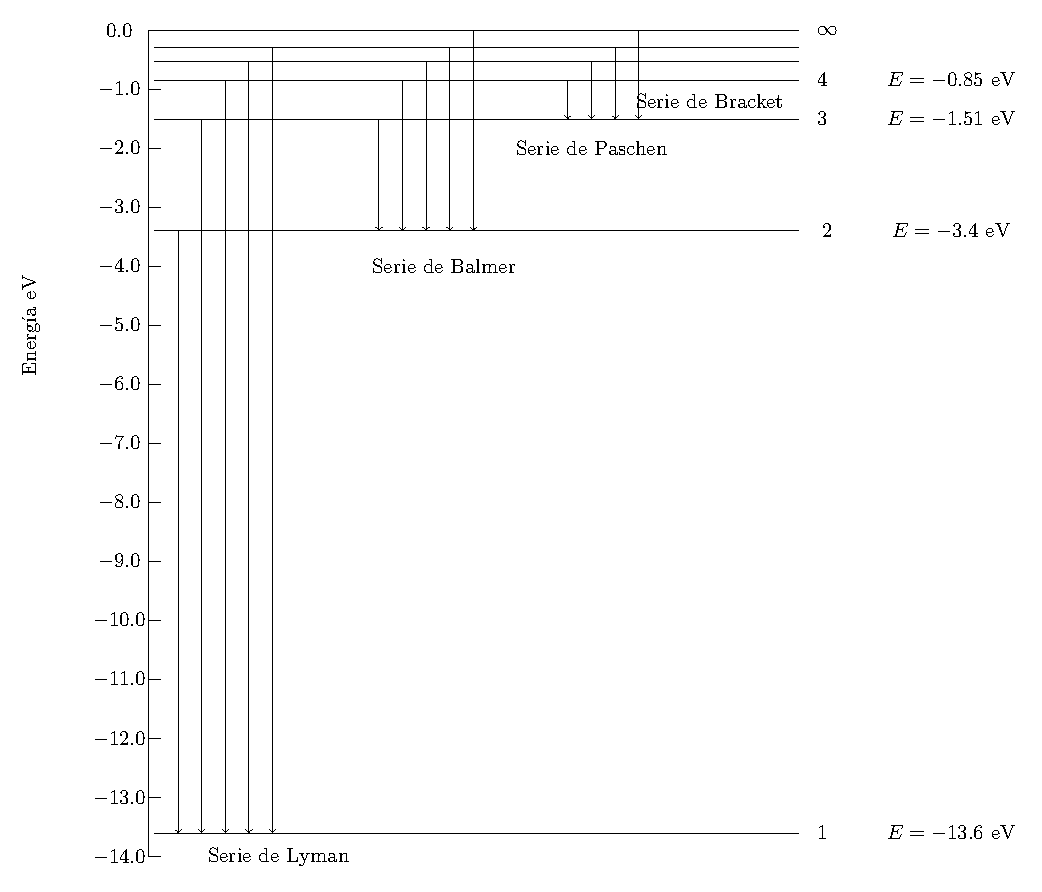
\includegraphics[scale=0.8]{Imagenes/espectrohidrogeno.eps}
    \caption{Niveles de energía y transiciones en el espectro de hidrógeno.}
    \label{fig:figura_espectro_H}
\end{figure}
\end{document}